\documentclass[10pt]{beamer}  % pour la présentation
%\documentclass[10pt,handout]{beamer}  % pour les notes de cours


\usetheme{Antibes}
\usecolortheme{whale}
\setbeamertemplate{navigation symbols}{}
\setbeamertemplate{mini frames}{} % Supprime les petits cercles dans le header
\setbeamertemplate{items}[triangle]
\setbeamercolor{itemize item}{fg=black}
\setbeamercolor{itemize subitem}{fg=gray}
\setbeamertemplate{frametitle continuation}{}


\usepackage[utf8]{inputenc}
\usepackage[T1]{fontenc}
\usepackage[french]{babel}
\usepackage{amsmath, amssymb}
\usepackage{hyperref}
\usepackage{graphicx}
\usepackage{caption}
\usepackage{tikz}
\usetikzlibrary{shapes.geometric, positioning}
\usepackage{nicematrix}
\usepackage{fontawesome5}
\usepackage{listings}
\usepackage{xcolor}

\lstset{
	language=Python,
	basicstyle=\ttfamily\small,
	keywordstyle=\color{blue},
	stringstyle=\color{red},
	commentstyle=\color{green!50!black},
	numbers=none, %left
	frame=single,
	breaklines=true,
	xleftmargin=0pt,
	literate={_}{\_}{1},
	columns=fixed,
	showstringspaces=false
}

%\newcommand{\Var}[1]{\mathbb{V}\mathrm{ar}\left[ #1 \right]}
%\newcommand{\Cov}[1]{\mathbb{C}\mathrm{ov}\left[ #1 \right]}
\newcommand{\E}[2][]{\operatorname{\mathbb{E}}_{#1}\left[#2\right]}
\newcommand{\Var}[1]{\operatorname{\mathbb{V}ar}\left[#1\right]}
\newcommand{\Cov}[1]{\operatorname{\mathbb{C}ov}\left[#1\right]}
\newcommand{\sigeps}{\sigma_{\epsilon}^2}
\newcommand{\ET}[1][]{\operatorname{ET}\ifx&#1&\else\left[#1\right]\fi}
\newcommand{\diag}{\operatorname{diag}}
\newcommand{\cote}{\operatorname{cote}}
\newcommand{\score}[1]{\operatorname{score}\left(#1\right)}
\newcommand{\logit}[1]{\operatorname{logit}\left(#1\right)}
\newcommand{\R}{\operatorname{\mathbb{R}}}
\newcommand{\argmax}[1]{\underset{#1}{\operatorname{arg\,max}}}

\title{Apprentissage Automatique - L3 - KMAXPP05}
\subtitle{Chapitre 2 : Algorithme Bayésien Naïf}
\author{Cédric Campguilhem}
\institute[]{
	Airbus Operations \\
	\href{mailto:cedric.campguilhem@airbus.com}{\texttt{cedric.campguilhem@airbus.com}}
}
\date{2025-2026}

\begin{document}
	
\begin{frame}
	\titlepage
\end{frame}

%=======================================================================================

\section[Introduction]{Introduction}

\begin{frame}{Algorithme Bayésien Naïf}
	L'algorithme Bayésien Naïf est un algorithme d'apprentissage \textbf{supervisé} utilisé pour résoudre des problèmes de \textbf{classification}. \\
	\pause
	\vspace{0.5cm}
	\begin{itemize}
		\item Il repose sur le \textbf{théorème de Bayes}...
		\pause
		\item ...avec quelques ajustements qui lui valent sa qualification de \textbf{naïf}.
	\end{itemize}
\end{frame}

\begin{frame}{Plan du cours}
	Au sommaire de ce cours:
	\begin{itemize}
		\item Rappels sur le théorème de Bayes
		\item Algorithme Bayésien Naïf
		\item Traitements simples de données textuelles
	\end{itemize}
\end{frame}

%=======================================================================================

\section[Rappels]{Rappels}

\subsection{Probabilité conditionnelle}

\begin{frame}{Probabilité conditionnelle}
	Le théorème de Bayes découle naturellement de la définition d'une probabilité conditionnelle:
	\begin{block}{Définition: probabilité conditionnelle}
		\'Etant donné deux événements $A$ et $B$, on définit la probabilité conditionnelle de $A \mid B$, qui se lit \textit{A sachant B}, comme le rapport entre la probabilité jointe de $A$ \textbf{et} $B$ et la probabilité marginale de $B$:
		\begin{equation}
			P(A \mid B) = \displaystyle \frac{P(A \cap B)}{P(B)}
			\nonumber
		\end{equation}
	\end{block}
\end{frame}

\begin{frame}{Probabilité conditionnelle}
	Lorsque les événements $A$ et $B$ sont indépendants, on peut écrire:
	\begin{equation}
		P(A \cap B) = P(A) \, P(B)
		\nonumber
	\end{equation}
	\pause
	La probabilité conditionnelle devient alors:
	\begin{equation}
		P(A \mid B) = \displaystyle \frac{P(A \cap B)}{P(B)} = \displaystyle \frac{P(A) \, P(B)}{P(B)} = P(A)
		\nonumber
	\end{equation}
	La connaissance de B ne change pas notre connaissance de A. \\
	\pause
	\vspace{0.3cm}
	La probabilité jointe $A \cap B$ est commutative donc:
	\begin{equation}
		P(A \cap B) = P(B \cap A)
		\nonumber
	\end{equation}
	\pause
	On note parfois la probabilité jointe de la façon suivante:
	\begin{equation}
		P(A \cap B) \equiv P(A, B)
		\nonumber
	\end{equation}
\end{frame}

\subsection{Théorème de Bayes}

\begin{frame}{Démonstration du théorème de Bayes}
	\`A partir des propriétés des probabilités conditionnelles et jointes on peut écrire:
	\begin{equation}
		P(A \mid B) \, P(B) = P(A \cap B) = P(B \cap A) = P(B \mid A) \, P(A)
		\nonumber
	\end{equation}
	Et donc:
	\begin{equation}
		P(A \mid B) = \frac{P(B \mid A) \, P(A)}{P(B)}
		\nonumber
	\end{equation}
\end{frame}

\begin{frame}{Théorème de Bayes}
	\begin{block}{Théorème de Bayes}
		Le théorème de Bayes permet, pour deux événements $A$ et $B$, de calculer la probabilité \textbf{a posteriori} de $A \mid B$ à partir de la \textbf{vraisemblance} de $B \mid A$, de la probabilité \textbf{a priori} de $A$ et de la probabilité \textbf{marginale} de $B$:
		\begin{equation}
			P(A \mid B) = \displaystyle \frac{P(B \mid A) \, P(A)}{P(B)}
			\nonumber
		\end{equation}
		\hfill
		\textit{--- Thomas Bayes (1763)}
	\end{block}
	\pause
	Ce théorème a donné naissance à un nouveau paradigme dans l'analyse des probabilités en venant en complément les méthodes \textbf{fréquentistes}. Mais il est aussi le fondement de certaines méthodes d'apprentissage automatique (comme les processus Gaussiens) ou en analyse de données (filtres de Kalman). 
\end{frame}

\subsection{Marginalisation}

\begin{frame}{Variable aléatoire discrète}
	Si l'événement $A$ est une variable aléatoire discrète, par exemple $A \in \{0, 1\}$, alors on peut écrire:
	\begin{equation}
		\begin{aligned}
			P(B) &= P(B \cap A=1) + P(B \cap A=0) \\
			     &= P(B \mid A=1) \, P(A=1) + P(B \mid A=0) \, P(A=0)
		\end{aligned}
		\nonumber 
	\end{equation}
	\pause
	Ou dans une forme plus générale si $A \in \{A_0, A_1, \cdots, A_k\}$:
	\begin{equation}
		\begin{aligned}
			P(B) &= \sum_{i=0}^k P(B \mid A=A_i) \, P(A=A_i) \\
			     &= \E[A]{P(B \mid A)}
		\end{aligned}
		\nonumber
	\end{equation}
	\pause
	Cette équation représente la \textbf{marginalisation} de $B$, c'est à dire la probabilité de $B$ exprimée en fonction de l'ensemble des valeurs possibles de l'événement $A$.
\end{frame}

\begin{frame}{Variable aléatoire continue}
	Si l'événement $A$ est une variable aléatoire continue $A \in \mathbb{R}$ alors la marginalisation de $B$ prend une forme intégrale équivalente:
	\begin{equation}
		\begin{aligned}
			P(B) &= \int_{-\infty}^{+\infty} P(B \mid A=x) f_A(x) dx \\
			     &= \E[A]{P(B \mid A)}
		\end{aligned}
		\nonumber
	\end{equation}
	Où $f_A$ représente la fonction de densité de probabilité de $A$.
\end{frame}

\subsection{Exemple}

\begin{frame}{Caractéristiques d'un test PCR pour la Covid 19}
	\faExclamationTriangle Les données dans cet exemple sont représentatives mais ne constituent pas une source fiable d'information sur la Covid 19. \\
	\vspace{0.5cm}
	\pause
	On considèrera les données suivantes pour un test PCR pour la Covid 19:
	\begin{itemize}
		\item La \textbf{sensibilité} du test est de 96\%. Cela signifie qu'un test PCR pour une personne atteinte de la maladie a 96\% de chance d'être positif. C'est aussi le \textbf{rappel} du test.
		\pause
		\item La \textbf{spécificité} du test est de 99\%. Cela signifie qu'un test PCR pour une personne qui n'est pas atteinte de la maladie a 99\% de chance d'être négatif.
		\pause
		\item On estime qu'en période de crise, la \textbf{prévalence} de la maladie pouvait être de 3\%.
		\pause
		\item En période d'accalmie, on considèrera une \textbf{prévalence} de 0.1\%.
	\end{itemize}
\end{frame}

\begin{frame}{Période de crise}
	En période de crise, supposons que nous avons un test positif. Quelle est la probabilité d'avoir la Covid 19 avec un test positif ?
	\begin{itemize}
		\item La probabilité a priori d'avoir la Covid 19: $P(C) = 0.03$. 
		\item La sensibilité du test est de 96\% donc: $P(T \mid C) = 0.96$.
		\item La spécificité du test est de 99\% donc: $P(\bar{T} \mid \bar{C}) = 0.99$.
	\end{itemize}
	\vspace{0.5cm}
	\pause
	Faisons un raisonnement rapide pour un groupe de 1000 personnes:
	\begin{itemize}
		\item Il y a 30 personnes infectées. On supposera qu'elles ont toutes un test positif.
		\pause
		\item Il y a 970 personnes non-infectées. Comme il y a 1\% d'avoir un faux positif, cela fait environ 10 personnes à avoir un faux positif.
		\pause
		\item Il y a donc 40 personnes avec un test positif. Et seulement 10 d'entre elles ne sont pas infectées. Cela signifie donc qu'une personne avec un test positif a approximativement 75\% de chance d'être infectée.
	\end{itemize}
\end{frame}

\begin{frame}{Période de crise - Calcul}
	La probabilité marginale est:
	\begin{equation}
		\begin{aligned}
			P(T) &= P(T \cap C) + P(T \cap \bar{C}) \\
			&= P(T \mid C) P(C) + P(T \mid \bar{C}) P(\bar{C}) \\
			&= P(T \mid C) P(C) + (1 - P(\bar{T} \mid \bar{C})) (1 - P(C)) \\
			&= 0.96 \times 0.03 + (1 - 0.99) \times (1 - 0.03) \\
			&= 0.0288 + 0.0097 = 0.0385
		\end{aligned}
		\nonumber
	\end{equation}
	\pause
	On peut donc calculer la probabilité a posteriori:
	\begin{equation}
		\begin{aligned}
			P(C \mid T) &= \frac{P(T \mid C) P(C)}{P(T)} \\
			&= \frac{0.96 \times 0.03}{0.0385} 
			= \frac{0.0288}{0.0385} \\
			&\approx 0.748
		\end{aligned}
		\nonumber
	\end{equation}
\end{frame}

\begin{frame}{Période de crise - Visualisation}
	\begin{figure}
		\centering
		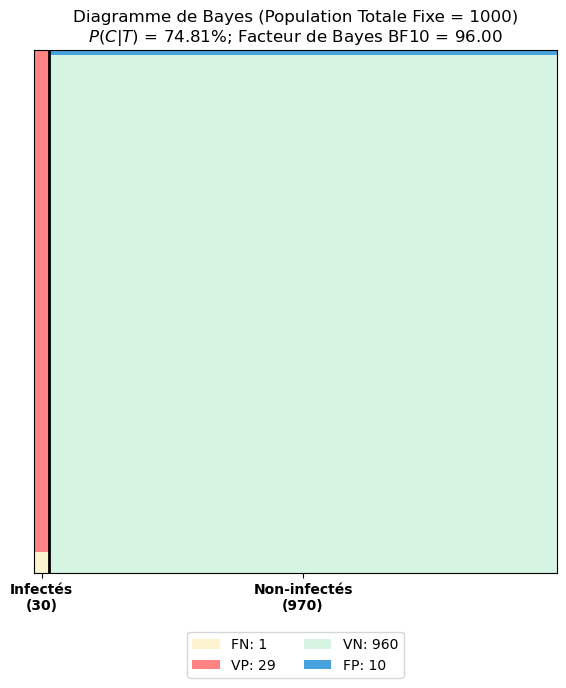
\includegraphics[width=0.5\linewidth]{Images/diagramme_bayes_crise}
		\label{fig:diagramme_bayes_crise}
	\end{figure}
\end{frame}

\begin{frame}{Période d'accalmie}
	En période d'accalmie, supposons que nous avons un test positif. Quelle est la probabilité d'avoir la Covid 19 avec un test positif ?
	\begin{itemize}
		\item La probabilité a priori d'avoir la Covid 19: $P(C) = 0.001$. 
		\item La sensibilité du test est de 96\% donc: $P(T \mid C) = 0.96$.
		\item La spécificité du test est de 99\% donc: $P(\bar{T} \mid \bar{C}) = 0.99$.
	\end{itemize}
	\vspace{0.5cm}
	\pause
	Faisons un raisonnement rapide pour un groupe de 1000 personnes:
	\begin{itemize}
		\item Il y a une personne infectée. On supposera que cette personne a un test positif.
		\pause
		\item Il y a 999 personnes non-infectées. Comme il y a 1\% d'avoir un faux positif, cela fait environ 10 personnes à avoir un faux positif.
		\pause
		\item Il y a donc 11 personnes avec un test positif. Et 10 d'entre elles ne sont pas infectées. Cela signifie donc qu'une personne avec un test positif a approximativement 9\% de chance d'être infectée.
	\end{itemize}
\end{frame}

\begin{frame}{Période d'accalmie - Calcul}
	La probabilité marginale est:
	\begin{equation}
		\begin{aligned}
			P(T) &= P(T \cap C) + P(T \cap \bar{C}) \\
			     &= P(T \mid C) P(C) + P(T \mid \bar{C}) P(\bar{C}) \\
			     &= P(T \mid C) P(C) + (1 - P(\bar{T} \mid \bar{C})) (1 - P(C)) \\
			     &= 0.96 \times 0.001 + (1 - 0.99) \times (1 - 0.001) \\
			     &= 0.00096 + 0.00999 = 0.01095
		\end{aligned}
		\nonumber
	\end{equation}
	\pause
	On peut donc calculer la probabilité a posteriori:
	\begin{equation}
		\begin{aligned}
			P(C \mid T) &= \frac{P(T \mid C) P(C)}{P(T)} \\
			            &= \frac{0.96 \times 0.001}{0.01095} 
			            = \frac{0.00096}{0.01095} \\
			            &\approx 0.088
		\end{aligned}
		\nonumber
	\end{equation}
\end{frame}

\begin{frame}{Période d'accalmie - Visualisation}
	\begin{figure}
		\centering
		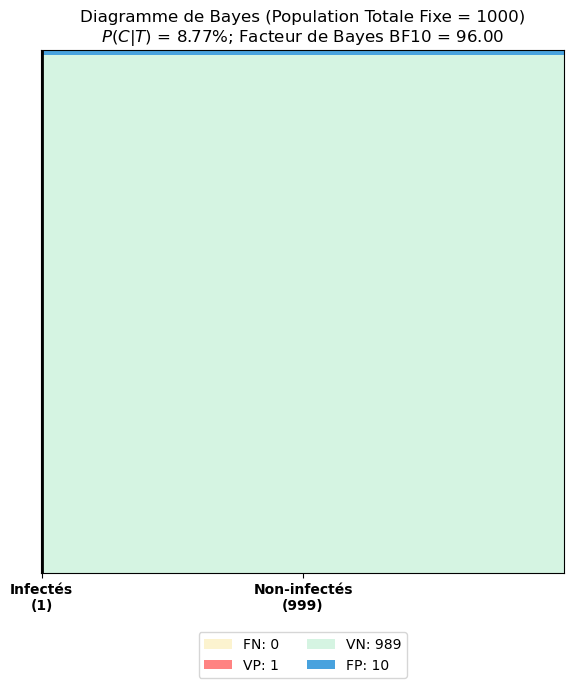
\includegraphics[width=0.5\linewidth]{Images/diagramme_bayes_accalmie}
		\label{fig:diagramme_bayes_accalmie}
	\end{figure}
\end{frame}


\begin{frame}{Période d'accalmie avec un second test positif}
	En période d'accalmie, supposons que nous avons un \textbf{second} test positif. On suppose ce test indépendant du premier. Quelle est la probabilité d'avoir la Covid 19 avec un second test positif ?
	\begin{itemize}
		\item La probabilité a priori d'avoir la Covid 19: $P(C) = 0.088$. C'est la probabilité d'avoir la Covid 19 après un premier test positif.
		\item La sensibilité du test est de 96\% donc: $P(T \mid C) = 0.96$.
		\item La spécificité du test est de 99\% donc: $P(\bar{T} \mid \bar{C}) = 0.99$.
	\end{itemize}
\end{frame}

\begin{frame}{Période d'accalmie avec un second test positif - Calcul}
	La probabilité marginale est:
	\begin{equation}
		\begin{aligned}
			P(T) &= P(T \cap C) + P(T \cap \bar{C}) \\
			&= P(T \mid C) P(C) + P(T \mid \bar{C}) P(\bar{C}) \\
			&= P(T \mid C) P(C) + (1 - P(\bar{T} \mid \bar{C})) (1 - P(C)) \\
			&= 0.96 \times 0.088 + (1 - 0.99) \times (1 - 0.088) \\
			&= 0.08448 + 0.00912 = 0.0936
		\end{aligned}
		\nonumber
	\end{equation}
	\pause
	On peut donc calculer la probabilité a posteriori:
	\begin{equation}
		\begin{aligned}
			P(C \mid T) &= \frac{P(T \mid C) P(C)}{P(T)} \\
			&= \frac{0.96 \times 0.088}{0.0936} 
			= \frac{0.08448}{0.0936} \\
			&\approx 0.903
		\end{aligned}
		\nonumber
	\end{equation}
\end{frame}

\subsection{Facteur de Bayes}

\begin{frame}{Introduction d'une forme alternative}
	Nous avons vu que le théorème de Bayes pour deux événements $A$ et $B$ s'écrit:
	\begin{equation}
		P(A \mid B) = \frac{P(B \mid A) P(A)}{P(B)}
		\nonumber
	\end{equation}
	\pause
	D'une manière similaire, on peut écrire:
	\begin{equation}
		P(\bar{A} \mid B) = \frac{P(B \mid \bar{A}) P(\bar{A})}{P(B)}
		\nonumber
	\end{equation}
	\pause
	En divisant ces deux relations:
	\begin{equation}
		\frac{P(A \mid B)}{P(\bar{A} \mid B)} = \frac{\frac{P(B \mid A) P(A)}{P(B)}}{\frac{P(B \mid \bar{A}) P(\bar{A})}{P(B)}}
		\nonumber
	\end{equation}	
\end{frame}

\begin{frame}{Facteur de Bayes}
	L'expression précédente se simplifie en:
	\begin{equation}
		\frac{P(A \mid B)}{P(\bar{A} \mid B)} = \frac{P(B \mid A)}{P(B \mid \bar{A})} \frac{P(A)}{P(\bar{A})}
		\nonumber
	\end{equation}
	\begin{block}{Définition: Facteur de Bayes}
		Soient deux événements $A$ et $B$, le facteur de Bayes est défini par:
		\begin{equation}
			\begin{cases}
				\text{BF}_{10}(B) = \displaystyle \frac{P(B \mid A)}{P(B \mid \bar{A})} \\[10pt]
				\text{BF}_{10}(\bar{B}) = \displaystyle \frac{P(\bar{B} \mid A)}{P(\bar{B} \mid \bar{A})}
			\end{cases}
			\nonumber
		\end{equation}
	\end{block}
	Note: l'indice $10$ signifie que la condition $A$ est vraie dans le numérateur et qu'elle est fausse dans le dénominateur. On aurait pu tout aussi bien définir un facteur de Bayes $\text{BF}_{01}$.
\end{frame}

\begin{frame}{Forme alternative du théorème de Bayes}
	En utilisant le facteur de Bayes, nous avons une forme alternative du théorème de Bayes utilisant les cotes:
	\begin{equation}
		\cote(A \mid B) = \text{BF}_{10}(B) \, \cote(A)
		\nonumber
	\end{equation}
	\pause
	Nous pouvons appliquer cette formulation pour notre problème de la Covid 19. Comme la sensibilité est de 96\% et la spécificité est de 99\%, on peut calculer le facteur de Bayes:
	\begin{equation}
		\begin{aligned}
			\text{BF}_{10}(T) &= \frac{P(T \mid C)}{P(T \mid \bar{C})} \\
			                  &= \frac{P(T \mid C)}{1 - P(\bar{T} \mid \bar{C})} \\
			                  &= \frac{0.96}{1 - 0.99} \\
			                  &= 96
		\end{aligned}
		\nonumber
	\end{equation}
\end{frame}

\begin{frame}{Forme alternative du théorème de Bayes}
	Nous pouvons utiliser ce facteur de Bayes pour résoudre les problèmes précédents. Il nous suffit de calculer la cote associée à la probabilité a priori. On rappelle que:
	\begin{equation}
		\cote = \frac{p}{1 - p}  \Longleftrightarrow p = \frac{\cote}{\cote + 1}
		\nonumber
	\end{equation}
	\begin{itemize}
		\item Si la probabilité a priori est de 3\%, la cote est $3:97$, et donc la cote a posteriori est $288:97$. Ce qui donne une probabilité a posteriori de 0.748.
		\item Si la probabilité a priori est de 0.1\%, la cote est $1:999$, et donc la cote a posteriori est $96:999$. Ce qui donne une probabilité a posteriori de 0.088.
		\item Si la probabilité a priori est de 8.8\%, la cote est $11:114$, et donc la cote a posteriori est $1056:114$. Ce qui donne une probabilité a posteriori de 0.903.
	\end{itemize}
\end{frame}

\subsection{Nature récursive du théorème de Bayes}

\begin{frame}{Critiques de cinéma}
	Un nouveau film vient de sortir au cinéma. On représentera notre avis par une variable aléatoire $A$ qui vaut 0 si on a un avis négatif sur le film et 1 sinon. Comme nous n'avons aucun avis précis sur le film, nous représenterons notre avis \textbf{a priori} par la fonction de masse suivante:
	\begin{equation}
		\begin{cases}
			P(A = 0) = 0.5 \\
			P(A = 1) = 0.5
		\end{cases}
		\nonumber
	\end{equation}
	\pause
	Nous lisons ensuite une série de critiques $C$, que l'on suppose indépendantes, qui peuvent être soit négatives $C=0$, soit positives $C=1$. Il nous faut aussi définir une sensibilité et une spécificité:
	\begin{itemize}
		\item \textbf{Sensibilité}: probabilité que la critique soit positive pour un film sur lequel on aurait un avis positif: 0.65
		\item \textbf{Spécificité}: probabilité que la critique soit négative pour un film sur lequel on aurait un avis négatif: 0.75
	\end{itemize}
\end{frame}

\begin{frame}{Critiques de cinéma - Visualisation}
	\begin{columns}
		\begin{column}{0.45\textwidth}
			Après avoir lu 2 critiques négatives et 2 critiques positives, nous avons maintenant un avis légèrement favorable sur le film. Pour obtenir ce résultat nous avons appliqué le théorème de Bayes 4 fois consécutives en utilisant la probabilité a posteriori du calcul précédent comme la probabilité a priori du calcul courant:
		\end{column}
		\begin{column}{0.55\textwidth}
			\begin{figure}
				\centering
				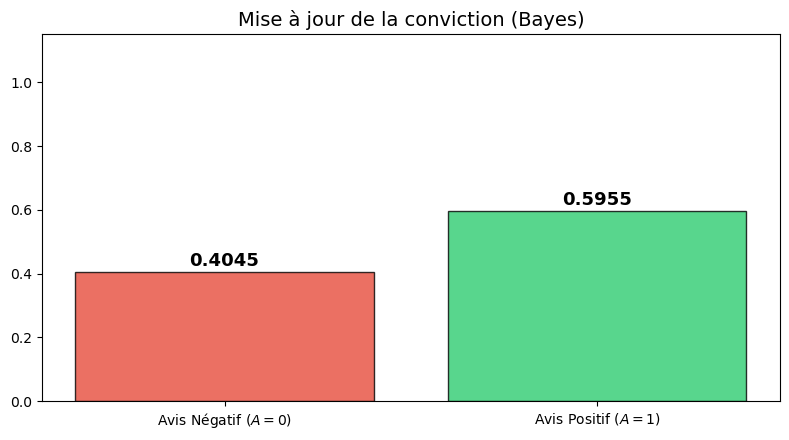
\includegraphics[width=1.0\linewidth]{Images/bayes_recursif}
				\label{fig:bayes_recursive}
			\end{figure}
		\end{column}		
	\end{columns}
	\vspace{0.5cm}
	Note: utiliser les facteurs de Bayes $\text{BF}_{10}(C=1)$ et $\text{BF}_{10}(C=0)$ rend le problème très rapide à résoudre:
	\begin{equation}
		\cote_{finale} = \text{BF}_{10}(C=0)^2 \text{BF}_{10}(C=1)^2 \cote_{initiale}
		\nonumber
	\end{equation}
\end{frame}

\subsection{Conclusion}

\begin{frame}{L'essentiel du raisonnement bayésien}
	L'inférence bayésienne n'est pas qu'une formule, c'est une \textbf{méthode de mise à jour des connaissances}.
	\vspace{0.3cm}
	\begin{itemize}
		\item \textbf{Le poids du contexte} : La probabilité \textit{a posteriori} dépend autant de la qualité de la preuve (vraisemblance) que de ce que l'on savait avant (a priori). 
		\begin{itemize}
			\item[$\rightarrow$] \textit{Un test excellent sur une maladie rare produit surtout des faux positifs.}
		\end{itemize}
		\pause
		\item \textbf{Le Facteur de Bayes ($BF_{10}$)} : C'est le multiplicateur de conviction. Il mesure la force intrinsèque d'une donnée, indépendamment du contexte.
		\pause
		\item \textbf{La nature récursive} : L'\textit{a posteriori} d'aujourd'hui est l'\textit{a priori} de demain. C'est le principe de l'apprentissage continu.
	\end{itemize}
\end{frame}

%=======================================================================================

\section[Algorithme Bayésien Naïf]{Algorithme Bayésien Naïf}

\subsection[Cas d'utilisation]{Cas d'utilisation}

\begin{frame}{Présentation du cas d'utilisation}
	Nous allons utiliser comme support des données textuelles: des critiques de films, afin de réaliser une \textbf{analyse de sentiment}.
	\begin{itemize}
		\item Nous allons utiliser une base de données de critiques de films postées par les utilisateurs du site anglophone \href{https://m.imdb.com/}{IMDb}: \url{https://www.kaggle.com/datasets/yasserh/imdb-movie-ratings-sentiment-analysis}
		\item Ces critiques sont soit positives, soit négatives.
		\item Nous allons donc construire un classifieur binaire pour associer une critique à une opinion (positive ou négative).
	\end{itemize}
	Un algorithme Bayésien Naïf est un très bon candidat pour ce genre de problème ! 
\end{frame}

\begin{frame}{Challenge}
	Il y a donc un double challenge !
	\begin{itemize}
		\item Comment traite-t-on des données textuelles avec un algorithme d'apprentissage automatique ?
		\item Comment est-ce qu'on peut utiliser le théorème de Bayes avec ces données ?
	\end{itemize}
\end{frame}

\begin{frame}{Données de travail}
	Supposons que nous avons collecté des exemples de critiques positives et négatives. Nous avons \textbf{compté} combien de fois certains mots apparaissent dans les critiques:
	\begin{columns}
		\begin{column}{0.5\textwidth}
			\begin{figure}
				\centering
				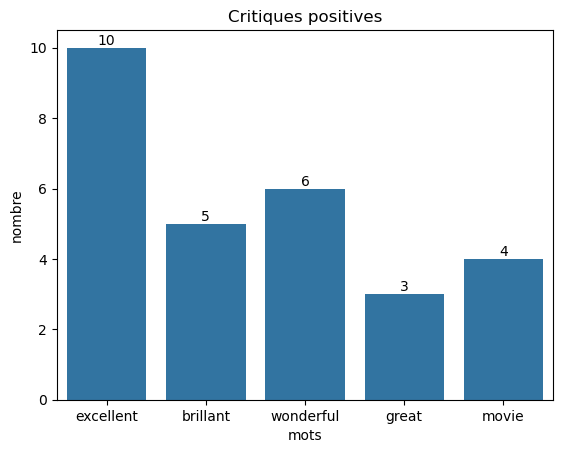
\includegraphics[width=1.0\linewidth]{Images/critiques_positives}
				\label{fig:critiques_positives}
			\end{figure}
		\end{column}
		\begin{column}{0.5\textwidth}
			\begin{figure}
				\centering
				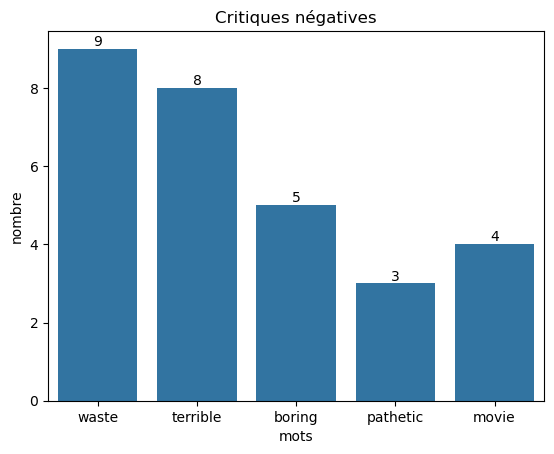
\includegraphics[width=1.0\linewidth]{Images/critiques_negatives}
				\label{fig:critiques_negatives}
			\end{figure}
		\end{column}		
	\end{columns}	
\end{frame}

\begin{frame}{Données de travail - Probabilités}
	Nous pouvons facilement en dériver des \textbf{probabilités conditionnelles}. Elles sont conditionnelles dans le sens où on traite séparément les critiques positives et les critiques négatives:
	\begin{columns}
		\begin{column}{0.5\textwidth}
			\begin{figure}
				\centering
				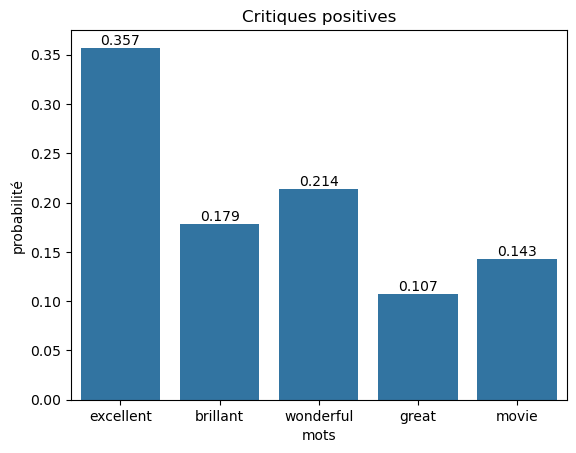
\includegraphics[width=1.0\linewidth]{Images/critiques_positives_probab}
				\label{fig:critiques_positives_probab}
			\end{figure}
		\end{column}
		\begin{column}{0.5\textwidth}
			\begin{figure}
				\centering
				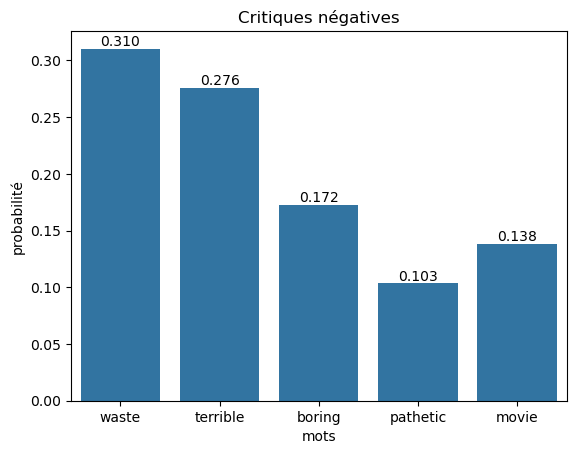
\includegraphics[width=1.0\linewidth]{Images/critiques_negatives_probab}
				\label{fig:critiques_negatives_probab}
			\end{figure}
		\end{column}		
	\end{columns}	
\end{frame}

\begin{frame}{Première tentative de calcul}
	\begin{itemize}
		\item Nous appellerons $C$ la variable aléatoire discrète $C \in \{0, 1\}$ qui désigne le sentiment associée à une critique.
		\pause
		\item  $C$ vaut 1 si la critique est positive et 0 sinon.	Supposons que la probabilité a priori est équilibrée: $P(C = 0) = 0.5$ et $P(C = 1) = 0.5$.
		\pause
		\item La critique qui nous intéresse est la suivante: \textit{brilliant}. Comment calculer une probabilité a posteriori ?
	\end{itemize}
	\pause
	Une façon de faire serait de calculer le facteur de Bayes:
	\begin{equation}
		\text{BF}_{10}(\text{"brilliant"}) = \frac{P(\text{"brilliant"} \mid C = 1)}{P(\text{"brilliant"} \mid C = 0)}
		\nonumber
	\end{equation}
	Mais il y a un petit problème: $P(\text{"brilliant"} \mid C = 0) = 0$. On aurait donc un facteur de Bayes infini !
\end{frame}

\begin{frame}{Données de travail - Lissage de Laplace}
	Nous allons transformer les données en utilisant un \textbf{lissage de Laplace}. Au lieu de calculer les probabilités conditionnelles comme ceci:
	\begin{equation}
		P(\text{mot} \mid C = K) = \frac{\text{nombre d'occurrences de mot quand } C = K}{\text{nombre total d'occurrences quand }C = K}
		\nonumber
	\end{equation}
	\pause
	On va les calculer comme ceci:
	\begin{equation}
		\begin{split}
			&P(\text{mot} \mid C = K) = \\
			&\frac{\text{nombre d'occurrences de mot quand } C = K + \color{red}1}{\text{nombre total occurrences quand } C = K + \color{red} \text{nombre total de mots différents}}
		\end{split}
		\nonumber
	\end{equation}
	\pause
	Cela consiste simplement à ajouter chaque mot une fois à l'ensemble des classes (critique positive et critique négative).
\end{frame}

\begin{frame}{Données de travail - Lissage de Laplace}
	Une fois le lissage de Laplace appliqué, nous avons donc:
	\begin{columns}
			\begin{column}{0.5\textwidth}
					\begin{figure}
							\centering
							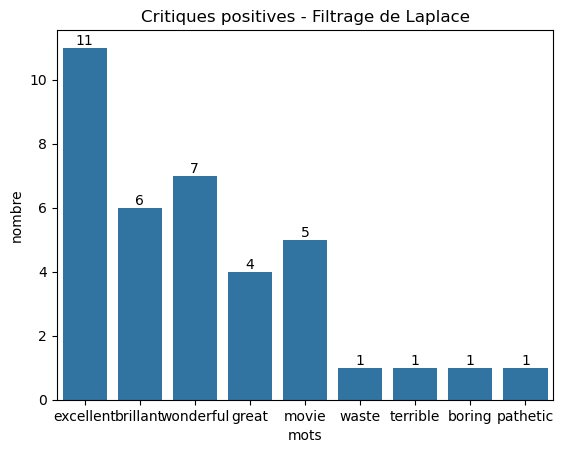
\includegraphics[width=1.0\linewidth]{Images/critiques_positives_laplace}
							\label{fig:critiques_positives_laplace}
						\end{figure}
				\end{column}
			\begin{column}{0.5\textwidth}
					\begin{figure}
							\centering
							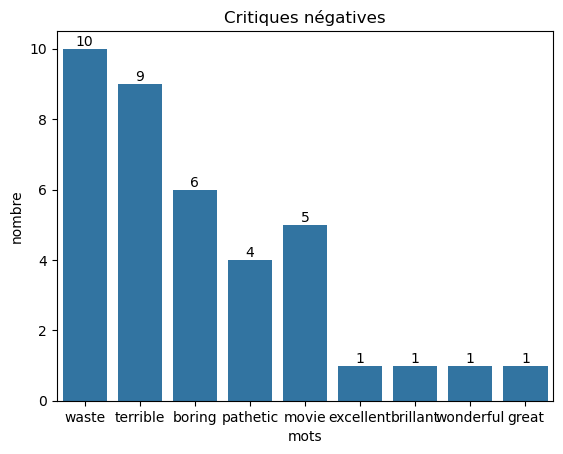
\includegraphics[width=1.0\linewidth]{Images/critiques_negatives_laplace}
							\label{fig:critiques_negatives_laplace}
						\end{figure}
				\end{column}		
		\end{columns}	
\end{frame}

\begin{frame}{Données de travail - Probabilités avec lissage de Laplace}
	Et les nouvelles probabilités conditionnelles:
	\begin{columns}
		\begin{column}{0.5\textwidth}
			\begin{figure}
				\centering
				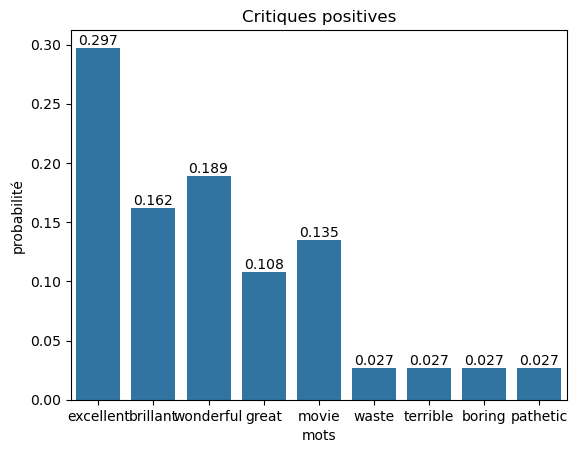
\includegraphics[width=1.0\linewidth]{Images/critiques_positives_probab_laplace}
				\label{fig:critiques_positives_probab_laplace}
			\end{figure}
		\end{column}
		\begin{column}{0.5\textwidth}
			\begin{figure}
				\centering
				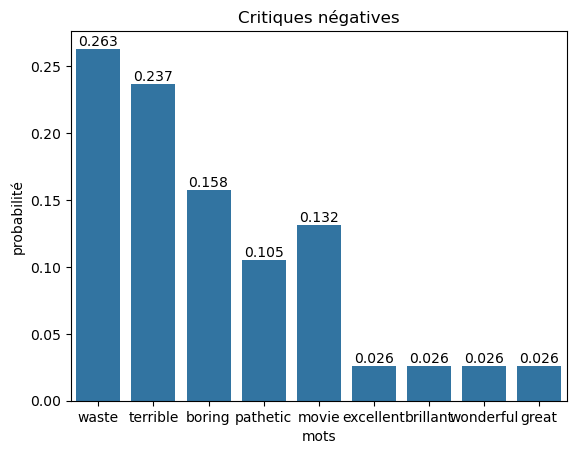
\includegraphics[width=1.0\linewidth]{Images/critiques_negatives_probab_laplace}
				\label{fig:critiques_negatives_probab_laplace}
			\end{figure}
		\end{column}		
	\end{columns}	
\end{frame}

\subsection[Calculs des probabilités]{Calculs des probabilités}

\begin{frame}{Premier calcul}
	\begin{itemize}
		\item  Supposons que la probabilité a priori est équilibrée: $P(C = 0) = 0.5$ et $P(C = 1) = 0.5$.
		\item La critique qui nous intéresse est la suivante: \textit{brilliant}. Comment calculer une probabilité a posteriori ?
	\end{itemize}
	\pause
	Une façon de faire serait de calculer le facteur de Bayes:
	\begin{equation}
		\begin{aligned}
			\text{BF}_{10}(\text{"brilliant"}) 
			&= \frac{P(\text{"brilliant"} \mid C = 1)}{P(\text{"brilliant"} \mid C = 0)} \\
			&= \frac{0.162}{0.026} \approx 6.23
		\end{aligned}
		\nonumber
	\end{equation}
	\pause
	La cote initiale étant de $1:1$, la cote finale devient $6.23:1$. Ce qui fait une probabilité a posteriori de 0.862.
\end{frame}

\begin{frame}{Premier calcul - Alternative}
	Une alternative consiste à calculer les 2 quantités suivantes qui correspondent aux numérateurs dans le théorème de Bayes:
	\begin{equation}
		\begin{cases}
			P(\text{"brilliant"} \mid C = 1) P(C=1) \\
			P(\text{"brilliant"} \mid C = 0) P(C=0)
		\end{cases}
		\nonumber
	\end{equation}
	\pause
	On ne s'embarrasse pas du dénominateur $P(\text{"brilliant"})$, vu que la somme des probabilités a posteriori doit être égale à 1:
	\begin{equation}
		\begin{cases}
			P(C = 1 \mid \text{"brilliant"}) \propto P(\text{"brilliant"} \mid C = 1) P(C=1) \\
			P(C = 0 \mid \text{"brilliant"}) \propto P(\text{"brilliant"} \mid C = 0) P(C=0)
		\end{cases}
		\nonumber
	\end{equation}
	C'est ce qui est implémenté dans l'algorithme Bayésien Naïf.
\end{frame}

\begin{frame}{Premier calcul - Alternative}
	On peut vérifier que cela mène au même résultat:
	\begin{equation}
		\begin{cases}
			P(\text{"brilliant"} \mid C = 1) P(C=1) = 0.162 \times 0.5 = 0.081 \\
			P(\text{"brilliant"} \mid C = 0) P(C=0) = 0.026 \times 0.5 = 0.013
		\end{cases}
		\nonumber
	\end{equation}	
	En normalisant, on obtient:
	\begin{equation}
		\begin{cases}
			P(C = 1 \mid \text{"brilliant"}) = 0.081 / (0.081 + 0.013) =  0.862 \\
			P(C = 0 \mid \text{"brilliant"}) = 0.013 / (0.081 + 0.013) =  0.138
		\end{cases}
		\nonumber
	\end{equation}
	On obtient, bien entendu, le même résultat. C'est la méthode implémentée dans un algorithme Bayésien Naïf.
\end{frame}

\subsection[Hypothèses de l'algorithme Bayésien Naïf]{Hypothèses de l'algorithme Bayésien Naïf}

\begin{frame}{Une critique plus élaborée}
	Supposons maintenant que la critique est \textit{boring movie, waste of time}:
	\begin{itemize}
		\item Les mots \text{of} et \text{time} ne font pas partie du \textbf{vocabulaire} que nous avons considéré.
		\pause
		\item Nous allons donc ignorer ces termes.
		\pause
		\item La ponctuation n'est pas non plus gérée. On va aussi s'en séparer. La critique est donc \textit{boring movie waste}.
		\pause
		\item Nous cherchons donc à calculer: $P(C = 1 \mid \text{"boring movie waste"})$ qui nécessite de connaitre la vraisemblance $P(\text{"boring movie waste"} \mid C = 1)$.
		\pause
		\item Mais nous ne connaissons pas la probabilité jointe de ces mots ! Ils sont forcément liés. Une phrase n'est pas juste un empilement de mots pris au hasard.
	\end{itemize}
	\pause
	C'est là que la nature \textbf{naïve} de l'algorithme intervient. Pour simplifier, on va considérer que les mots au sein d'une même phrase sont indépendants. C'est \textbf{faux} mais cela simplifie grandement les calculs !
\end{frame}

\begin{frame}{Nature naïve de l'algorithme}
	\begin{itemize}
		\item C'est là que la nature \textbf{naïve} de l'algorithme intervient.
		\pause
		\item Pour simplifier, on va considérer que les mots au sein d'une même phrase sont indépendants.
		\pause
		\item C'est \textbf{simpliste} mais bien pratique pour faire les calculs !
	\end{itemize}
	\pause
	\vspace{0.5cm}
	C'est comme dans tous les exemples traités jusqu'à maintenant. On a pris pour hypothèse que les tests Covid 19 étaient indépendants. De même que les critiques de films. Et ici on considère les mots au sein d'une même phrase comme indépendants !
\end{frame}

\begin{frame}{Nature multinomiale de l'algorithme}
	\begin{itemize}
		\item Rappel, notre critique simplifiée est: \textit{boring movie waste}.
		\pause
		\item On considère chaque mot comme indépendant. Donc Il s'agit de faire 3 mises à jour avec le théorème de Bayes, ou multiplier 3 facteurs de Bayes.
		\pause
		\item La différence avec nos exemples précédents c'est que chaque mot apporte une conviction \textbf{différente}: les facteurs de Bayes sont différents pour chaque mots, c'est la nouveauté.
		\pause
		\item C'est pour cette raison que cet algorithme est appelé algorithme Bayésien Naïf \textbf{multinomial}. 
		\pause
		\item Multinomial fait allusion à la nature de la distribution de probabilité. Nos exemples précédents utilisaient une distribution de Bernoulli !
		\pause
		\item Notre algorithme utilise 2 distributions multinomiales, une pour les critiques négatives et une pour les critiques positives. Les tracés graphiques avec les probabilités vus précédemment sont en fait les tracés des fonctions de masse de ces distributions. !
	\end{itemize}
\end{frame}

\begin{frame}{Une critique plus élaborée - Calcul}
	\begin{equation}
		\resizebox{1.0\textwidth}{!}{%
			$\begin{cases}
				P(C = 0 \mid \text{"boring movie waste"}) \propto P(\text{"boring movie waste"} \mid C = 0) P(C=0) \\
				P(C = 1 \mid \text{"boring movie waste"}) \propto P(\text{"boring movie waste"} \mid C = 1) P(C=1)
			\end{cases}$
		}
		\nonumber
	\end{equation}
	\pause
	Avec l'hypothèse d'indépendance naïve on peut écrire:
	\begin{equation}
		\begin{aligned}
			&P(\text{"boring movie waste"} \mid C = 0) P(C=0) \\
			&= P(\text{"boring"} \mid C = 0) P(\text{"movie"} \mid C = 0) P(\text{"waste"} \mid C = 0) P(C=0) \\
			&= 0.158 \times 0.132 \times 0.263 \times 0.5 \\
			&\approx 0.00274 
		\end{aligned}
		\nonumber
	\end{equation}
	\pause
	Similairement:
	\begin{equation}
		\begin{aligned}
			&P(\text{"boring movie waste"} \mid C = 1) P(C=1) \\
			&= P(\text{"boring"} \mid C = 1) P(\text{"movie"} \mid C = 1) P(\text{"waste"} \mid C = 1) P(C=1) \\
			&= 0.027 \times 0.135 \times 0.027 \times 0.5 \\
			&\approx 0.00005
		\end{aligned}
		\nonumber
	\end{equation}
\end{frame}

\begin{frame}{Une critique plus élaborée - Calcul}
	Après normalisation, on obtient:
	\begin{equation}
		\begin{cases}
			P(C = 0 \mid \text{"boring movie waste"}) \approx 0.982 \\
			P(C = 1 \mid \text{"boring movie waste"}) \approx 0.018
		\end{cases}
		\nonumber
	\end{equation}
	\pause
	Les probabilités qui se multiplient donnent très vite des nombres très petits. Les algorithmes calculent les \textbf{logarithmes} des probabilités. Grâce à l'hypothèse d'indépendance, le logarithme du produit des probabilités devient la somme des logarithmes des probabilités.
\end{frame}

\begin{frame}{Une critique plus élaborée - Facteurs de Bayes}
	On pourrait calculer les facteurs de Bayes pour chaque mot:
	\begin{equation}
		\begin{cases}
			\text{BF}_{10}(\text{"boring"}) = P(\text{"boring"} \mid C = 1) / P(\text{"boring"} \mid C = 0) \approx 0.171 \\
			\text{BF}_{10}(\text{"movie"}) = P(\text{"movie"} \mid C = 1) / P(\text{"movie"} \mid C = 0) \approx 1.023 \\
			\text{BF}_{10}(\text{"waste"}) = P(\text{"waste"} \mid C = 1) / P(\text{"waste"} \mid C = 0) \approx 0.103
		\end{cases}
		\nonumber
	\end{equation}
	\pause
	\begin{itemize}
		\item Le mot \textit{movie} aura très peu d'influence sur le résultat car son facteur de Bayes est très proche de 1.
		\item Le mot \textit{waste} est celui qui apporte la plus grande conviction que la critique est négative.
		\item On peut très facilement dériver les facteurs de Bayes en divisant les 2 fonctions de masse des distributions multinomiales.
	\end{itemize}
\end{frame}

\subsection[Formulation de l'algorithme Bayésien Naïf]{Formulation de l'algorithme Bayésien Naïf}

\begin{frame}{Hypothèse d'indépendance conditionnelle}
	Soient $x \in \R^d$ une caractéristique d'entrée et une variable aléatoire discrète $C \in \{0, 1\}$.
	\vspace{0.3cm}
	\begin{block}{Hypothèse d'indépendance conditionnelle (Naïve)}
		On suppose qu'il y a une indépendance conditionnelle dans les éléments de $x$:
		\begin{equation}
			P(x_1, x_2, \cdots, x_d \mid C = k) = \prod_{i=1}^{d} P(x_i \mid C = k) \quad k \in \{0, 1\}
			\nonumber
		\end{equation}
	\end{block}
\end{frame}

\begin{frame}{Maximum a posteriori}
	\begin{block}{Règle de décision (Maximum A Posteriori)}
		On cherche la classe qui maximise le produit de la probabilité a priori et de la vraisemblance:
		\begin{equation}
			\hat{y} = \argmax{k \in \{0, 1\}} \left( P(C = k) \prod_{i=1}^{d} P(x_i \mid C = k) \right)
			\nonumber
		\end{equation}
	\end{block}
	\pause
	Note: L'hypothèse naïve \textit{biaise} la probabilité a posteriori, mais comme nous ne recherchons que le maximum a posteriori, l'impact de cette hypothèse simpliste est limité sur les cas d'application.
\end{frame}

\begin{frame}{Passage au Logarithme}
	Pour éviter les erreurs de précision numérique et transformer les produits en sommes:
	\begin{block}{Règle de décision (Maximum A Posteriori)}
		On cherche la classe qui maximise le logarithme du produit de la probabilité a priori et de la vraisemblance:
		\begin{equation}
			\hat{y} = \argmax{k \in \{0, 1\}} \left( \ln P(C = k) + \sum_{i=1}^{d} \ln P(x_i \mid C = k) \right)
			\nonumber
		\end{equation}
	\end{block}
	\pause
	\begin{itemize}
		\item C'est l'implémentation de  \href{https://scikit-learn.org/stable/modules/generated/sklearn.naive_bayes.MultinomialNB.html}{\texttt{sklearn.naive\_bayes.MultinomialNB}}.
	\end{itemize}
\end{frame}

\begin{frame}{Calcul des probabilités avec la fonction softmax}
	Une fois les logarithmes $\ln P(C = k \mid x_1, \cdots, x_d)$ calculés, on peut calculer les probabilités avec une fonction \textbf{softmax}:
	\begin{equation}
		\resizebox{1.0\textwidth}{!}{%
		$P(C = 1 \mid x_1, \cdots, x_d) = \frac{\exp{\left(\ln P(C = 1  \mid x_1, \cdots, x_d)\right)}}{\exp{\left(\ln P(C = 1  \mid x_1, \cdots, x_d)\right)} + \exp{\left(\ln P(C = 0  \mid x_1, \cdots, x_d)\right)}}$
		}
		\nonumber
	\end{equation}
\end{frame}

\subsection[Combinaison d'algorithmes]{Combinaison d'algorithmes}

\begin{frame}{Cas d'étude}
	\begin{itemize}
		\item Sur le campus de l'université de Toulouse, à partir d'un échantillon d'étudiants et d'étudiantes on collecte la taille ainsi que l'UFR (Unité de Formation et de Recherche) comme Faculté de Santé, Lettres, Arts, Faculté des Sciences et de l'ingénierie.
		\pause
		\item On dispose de statistiques globales qui nous permettent de connaitre la répartition des étudiants (40\%) et des étudiantes (60\%). C'est notre probabilité a priori.
		\pause
		\item Nous pouvons établir deux distributions Gaussiennes pour la taille des étudiants et des étudiantes et utiliser ces distributions dans un algorithme Bayésien Naïf Gaussien.
		\pause
		\item Nous pouvons établir deux distributions multinomiales pour les UFR des étudiants et des étudiantes et utiliser ces distributions dans un algorithme Bayésien Naïf multinomial.
	\end{itemize}
\end{frame}

\begin{frame}{Cas d'étude - Calcul}
	\begin{itemize}
		\item Supposons que nous ayons un étudiant (ou une étudiante), dont nous connaissons la taille (172 cm) et l'UFR (Lettres). Quelle est la probabilité que ce soit une étudiante ?
		\pause
		\item On pourrait calculer les vraisemblances $\ln P(\text{Lettres} \mid \text{\'Etudiante})$ et $\ln P(\text{Lettres} \mid \text{\'Etudiant})$ en utilisant les distributions multinomiales. En fait, il s'agit de lire les fonctions de masse !
		\pause
		\item On pourrait calculer les vraisemblances $\ln P(\text{172 cm} \mid \text{\'Etudiante})$ et $\ln P(\text{172 cm} \mid \text{\'Etudiant})$ en utilisant les distributions Gaussiennes.
		\pause
		\item On ajoute ensuite ces vraisemblances à leur probabilité a priori: $\ln P(\text{Lettres} \mid \text{\'Etudiante}) + \ln P(\text{172 cm} \mid \text{\'Etudiante}) + \ln P(\text{\'Etudiante})$
		\pause
		\item Puis $\ln P(\text{Lettres} \mid \text{\'Etudiant}) + \ln P(\text{172 cm} \mid \text{\'Etudiant}) + \ln P(\text{\'Etudiant})$. 
		\pause
		\item On passe par la fonction softmax, et voilà !
	\end{itemize}
\end{frame}

\begin{frame}{Cas d'étude - Précisions pour l'algorithme Bayésien Naïf Gaussien}
	Pour une variable continue (taille), on ne compte plus des occurrences. On utilise la \textbf{loi normale}:
	\begin{equation}
		P(x \mid C=k) = \frac{1}{\sqrt{2\pi\sigma_k^2}} \exp\left(-\frac{(x-\mu_k)^2}{2\sigma_k^2}\right)
		\nonumber
	\end{equation}
	\pause
	\begin{itemize}
		\item $\mu_k$ : Taille moyenne de la classe $k$ (ex: 164 cm pour une étudiante, 176 cm pour un étudiant).
		\item $\sigma_k$ : \'Ecart-type de la classe $k$.
	\end{itemize}
	\pause
	\vspace{0.3cm}
	Le calcul en logarithme:
	\begin{equation}
		\ln P(x \mid C=k) = -\frac{1}{2} \ln(2\pi\sigma_k^2) - \frac{(x-\mu_k)^2}{2\sigma_k^2}
		\nonumber
	\end{equation}
	Plus l'étudiant(e) est proche de la moyenne, plus ce score est élevé.
\end{frame}

%=======================================================================================

\section[Traitements simples de données textuelles]{Traitements simples de données textuelles}

\subsection[Introduction]{Introduction}

\begin{frame}{Contenu}
	Ce cours n'a pas vocation à être très avancé sur le traitement des données textuelles. Mais nous introduirons les concepts suivants:
	\begin{itemize}
		\item Tokenisation et mots vides (stop words)
		\item Lemmatisation et analyse grammaticale (Part of Speech)
		\item Vectorisation
		\item TF-IDF (term frequency, inverse document frequency)
	\end{itemize}
	Nous illustrerons ces éléments sur le dataset d'analyse de sentiment \href{https://www.kaggle.com/datasets/yasserh/imdb-movie-ratings-sentiment-analysis}{IMDb}. Il existe des librairies disposant de fonctions pour traiter les textes en langue anglaise, comme \href{https://www.nltk.org/}{NLTK (Natural Language Toolkit)}.
\end{frame}

\subsection[Tokenisation]{Tokenisation}

\begin{frame}[fragile]{Tokenisation}
	La tokenisation consiste à découper une phrase en éléments simples, \textbf{tokens}. On en profite en général pour passer le texte en lettres minuscules et pour supprimer la ponctuation.\\
	
	Par exemple:
	\begin{lstlisting}
reviews = [
	"I loved every second of this masterpiece!",
	"The actors were terrible and the story was boring.",
	"Amazing music and great special effects!",
	"I would rather watch paint dry than see this movie.",
	"A complete waste of time and money!",
	"Don't miss this masterpiece!"
]
	\end{lstlisting}
\end{frame}

\begin{frame}[fragile]{Tokenisation}
	Donnerait les tokens suivants:
	\begin{lstlisting}
['i', 'loved', 'every', 'second', 'of', 'this', 'masterpiece']
['the', 'actors', 'were', 'terrible', 'and', 'the', 'story', 'was', 'boring']
['amazing', 'music', 'and', 'great', 'special', 'effects']
['i', 'would', 'rather', 'watch', 'paint', 'dry', 'than', 'see', 'this', 'movie']
['a', 'complete', 'waste', 'of', 'time', 'and', 'money']
['do', "n't", 'miss', 'this', 'masterpiece']
	\end{lstlisting}
	\vfill
	Méthodes: \href{https://www.nltk.org/api/nltk.tokenize.html\#nltk-tokenize-package}{\texttt{nltk.word\_tokenize}}
\end{frame}

\begin{frame}[fragile]{Tokenisation - Stop Words}
	NLTK dispose d'une liste de mots vides (stop words) qui n'apportent que peu ou pas de sens à la phrase. Ou alors qui sont tellement communs qu'on les retrouverait à la fois dans des critiques positives et négatives:
	\begin{lstlisting}
['loved', 'every', 'second', 'masterpiece']
['actors', 'terrible', 'story', 'boring']
['amazing', 'music', 'great', 'special', 'effects']
['would', 'rather', 'watch', 'paint', 'dry', 'see', 'movie']
['complete', 'waste', 'time', 'money']
["n't", 'miss', 'masterpiece']
	\end{lstlisting}
	\vfill
	Méthodes: \href{https://www.nltk.org/howto/corpus.html\#word-lists-and-lexicons}{\texttt{nltk.corpus.stopwords}}
\end{frame}

\subsection[Lemmatisation]{Lemmatisation}

\begin{frame}[fragile]{Lemmatisation}
	\begin{itemize}
		\item La \textbf{lemmatisation} est une technique qui consiste à remplacer un mot, par le mot que l'on trouverait dans un dictionnaire. Par exemple un mot pluriel deviendrait singulier. Un verbe conjugué prendrait une forme infinitive...
		\pause
		\item La tokenisation et les mots vides semblaient plus simples, la lemmatisation nécessite d'utiliser des bases de données pour connaitre les différents \textbf{lemmes} et leurs variantes.
		\pause
		\item Une autre difficulté et que la lemmatisation peut dépendre du contexte grammatical. Et donc de la langue ! C'est pour cette raison que l'on se repose sur des librairies qui implémentent tout ça pour nous, comme NLTK.
		\pause
		\item L'analyse grammaticale (\textbf{Part of Speech}) est réalisée par un outil. D'ailleurs il arrive que ce soit lui-même un outil d'apprentissage automatique, comme un réseau de neurones ou une chaine de Markov !
	\end{itemize}
\end{frame}

\begin{frame}[fragile]{Lemmatisation - POS}
	Part of Speech appliqué à notre exemple:
	\begin{lstlisting}
[('i', 'NN'), ('loved', 'VBD'), ('every', 'DT'), ('second', 'NN'), ('of', 'IN'), ('this', 'DT'), ('masterpiece', 'NN'), ('!', '.')]
[('the', 'DT'), ('actors', 'NNS'), ('were', 'VBD'), ('terrible', 'JJ'), ('and', 'CC'), ('the', 'DT'), ('story', 'NN'), ('was', 'VBD'), ('boring', 'VBG'), ('.', '.')]
	\end{lstlisting}
	Où nous retrouvons des noms singulier (NN) ou pluriel (NNS), des verbes (VBD), -parfois au gérondif (VBG)-, des déterminants (DT), de la ponctuation (.), des adjectifs (JJ), des conjonctions de coordination (CC). \\
	\vfill
	Méthodes: \href{https://www.nltk.org/api/nltk.stem.wordnet.html#nltk.stem.wordnet.WordNetLemmatizer}{\texttt{nltk.stem.wordnet.WordNetLemmatizer}}
\end{frame}

\begin{frame}[fragile]{Lemmatisation - POS}
	Après une lemmatisation utilisant POS:
	\begin{lstlisting}
['love', 'second', 'masterpiece']
['actor', 'terrible', 'story', 'bore']
['amazing', 'music', 'great', 'special', 'effect']
['rather', 'watch', 'paint', 'dry', 'see', 'movie']
['complete', 'waste', 'time', 'money']
["n't", 'miss', 'masterpiece']
	\end{lstlisting}
	Les mots sont maintenant uniquement singuliers et les verbes ont été remplacés par leur forme infinitive.
\end{frame}

\subsection[Vectorisation]{Vectorisation}

\begin{frame}{Vectorisation - Idée générale}
	Une fois les critiques tokénisées et lemmatisées, il est nécessaire de convertir ces données en \textbf{données numériques} pour qu'elles puissent être traitées par un algorithme d'apprentissage automatique. Cette opération peut être réalisée par une opération simple de \textbf{vectorisation par comptage}:
	\begin{itemize}
		\item L'idée consiste à établir une liste de $d$ tokens qui vont définir un \textbf{vocabulaire}.
		\item Chaque mot dans le vocabulaire est associé à un élément $i$ d'un vecteur.
		\item Chaque critique ayant été convertie en une liste de tokens, on compte combien de fois chaque token du vocabulaire est représenté dans la liste de tokens de la critique.
	\end{itemize}	
\end{frame}

\begin{frame}{Vocabulaire et Corpus}
	\begin{block}{Définition: vocabulaire}
		On appelle \textbf{vocabulaire} l'ensemble $V$ des $d$ tokens (ou mots) \textbf{uniques} présents dans les données d'apprentissage $\mathcal{D}$:
		\begin{equation}
			V = \{m_1, m_2, \cdots, m_d\}
			\nonumber
		\end{equation}
	\end{block}
	\pause
	\begin{block}{Définition: corpus}
		On appelle \textbf{corpus} l'ensemble $\mathcal{D}$ des $n$ documents textuels $t \in \mathcal{T}$  présents dans les données d'apprentissage:
		\begin{equation}
			\mathcal{D} = \{t^{(1)}, t^{(2)}, \cdots, t^{(n)}\}
			\nonumber
		\end{equation}
	\end{block}	
\end{frame}

\begin{frame}{Vectorisation par comptage - Formulation}
	\begin{block}{Vectorisation par comptage}
		La \textbf{vectorisation par comptage} consiste en une fonction $\Phi: \mathcal{T} \to \mathbb{N}^d$ qui permet de déterminer, pour un texte $i$, un vecteur $x^{(i)} \in \mathbb{N}^d$:
		\begin{equation}
			x^{(i)} = \Phi(t^{(i)}) = \begin{pmatrix}
				\text{tf}^{(i)}_1 &	\text{tf}^{(i)}_2 &	\cdots & \text{tf}^{(i)}_d
			\end{pmatrix}
			\nonumber
		\end{equation}
		Où $\text{tf}^{(i)}_j$ représente le nombre de fois (i.e. \textbf{fréquence du mot}) où le mot $m_j$ apparait dans le document textuel $t^{(i)}$. $\text{tf}^{(i)}_j$ peut aussi être décrite avec une \textbf{fonction indicatrice}:
		\begin{equation}
			\text{tf}^{(i)}_j = \underset{w \in t^{(i)}}{\sum} 1(w = m_j)
			\nonumber
		\end{equation}
		La fonction $1(u)$ vaut 1 si $u$ est une condition vraie et 0 sinon.
	\end{block}
	\vfill
	Méthodes: \href{https://scikit-learn.org/stable/modules/generated/sklearn.feature_extraction.text.CountVectorizer.html}{\texttt{sklearn.feature\_extraction.text.CountVectorizer}}
\end{frame}

\begin{frame}{Vectorisation avec TF-IDF}
	Le comptage simple donne trop d'importance aux mots fréquents. Le \textbf{TF-IDF} permet de pénaliser les mots communs à tout le corpus $\mathcal{D}$:
	\begin{block}{Calcul du score TF-IDF}
		Le score pour un mot $m_j$ dans un document $t^{(i)}$ est :
		\begin{equation}
			\text{tf-idf}_j^{(i)} = \text{tf}_j^{(i)} \times \ln\left( \frac{n}{n_{m_j}} \right)
			\nonumber
		\end{equation}
		Avec $n_{m_j}$ le nombre de documents contenant le mot $m_j$.
	\end{block}
	\begin{itemize}
		\item \textbf{TF}: Fréquence du mot dans le document ($\text{tf}^{(i)}_j$).
		\item \textbf{IDF}: Logarithme de l'inverse de la fréquence documentaire. Nul si $n_{m_j} = n$
	\end{itemize}
	\vfill
	Méthodes: \href{https://scikit-learn.org/stable/modules/generated/sklearn.feature_extraction.text.TfidfTransformer.html}{\texttt{sklearn.feature\_extraction.text.TfidfTransformer}} et \href{https://scikit-learn.org/stable/modules/generated/sklearn.feature_extraction.text.TfidfVectorizer.html}{\texttt{sklearn.feature\_extraction.text.TfidfVectorizer}}.
\end{frame}

\subsection[Calcul des probabilités]{Calcul des probabilités}

\begin{frame}{Calcul des probabilités}
	Le vocabulaire $V$ est le \textbf{même} pour toutes les classes. La vectorisation se fait pour chaque classe $k$ séparément à partir des données de la classe $\mathcal{D}_k$. Les probabilités sont calculées par l'algorithme \href{https://scikit-learn.org/stable/modules/generated/sklearn.naive_bayes.MultinomialNB.html}{\texttt{sklearn.naive\_bayes.MultinomialNB}}:
	\begin{block}{Calcul des probabilités avec lissage de Laplace}
		Les probabilités de la loi multinomiale sont calculées séparément pour chaque classe $k$ :
		\begin{equation}
			P(m_j \mid C = k) = \frac{1 + \underset{t^{(i)} \in \mathcal{D}_k}{\sum} \text{tf}^{(i)}_j}{d + \underset{t^{(i)} \in \mathcal{D}_k}{\sum} \sum_{j=1}^d \text{tf}^{(i)}_j}
			\nonumber
		\end{equation}
		Dans le cas où TF-IDF est utilisé, on remplace $\text{tf}^{(i)}_j$ par $\text{tf-idf}^{(i)}_j$.
	\end{block}
	\textit{Note : Le lissage ajoute virtuellement un document de $d$ tokens contenant chaque mot une fois.}
\end{frame}

%======================================================================================

\section{Conclusions}

\begin{frame}{Conclusions}
	Dans ce cours, nous avons fait des rappels de probabilités:
	\begin{itemize}
		\item Probabilités conditionnelles.
		\item Théorème de Bayes.
		\item Facteur de Bayes.
		\item Récursivité du théorème de Bayes.
	\end{itemize}
	\pause
	Nous avons également vu comme l'algorithme Bayésien Naïf utilisait le théorème de Bayes pour résoudre un problème de classification:
	\begin{itemize}
		\item Avec des données suivant une distribution multinomiale (données textuelles): algorithme Bayésien Naïf multinomial.
		\item Avec des données suivant une distribution Gaussienne: algorithme Bayésien Naïf Gaussien.
	\end{itemize}
	\pause
	Nous avons également vu que l'hypothèse de naïveté sur l'indépendance conditionnelle permettait de traiter des problèmes de classification avec des caractéristiques d'entrée suivant des distributions de différentes formes (multinomiale, Gaussienne...) en combinant plusieurs algorithmes Bayésiens Naïfs.
\end{frame}

\begin{frame}{Conclusions}
	Enfin nous avons introduit des techniques rudimentaires de traitements de données textuelles:
	\begin{itemize}
		\item Tokenisation et mots vides.
		\item Lemmatisation et analyse grammaticale.
		\item Vectorisation par comptage et TF-IDF.
	\end{itemize}
	\pause
	Ces traitements ne sont pas exclusifs aux algorithmes Bayésiens Naïfs et pourront être réutilisés pour d'autres algorithmes d'apprentissage automatique.
\end{frame}


%======================================================================================

\end{document}
